% -----------------------------------------------
% Template for SMC 2016
% adapted from the template for SMC 2012 and 2011, which were adapted from that of SMC 2010
% -----------------------------------------------

\documentclass{article}
\usepackage{smc2016}
\usepackage{times}
\usepackage{ifpdf}
\usepackage[english]{babel}
\usepackage{todonotes}
\usepackage{listings}
\usepackage{cite}
\usepackage{textcomp}

%%%%%%%%%%%%%%%%%%%%%%%% Some useful packages %%%%%%%%%%%%%%%%%%%%%%%%%%%%%%%
%%%%%%%%%%%%%%%%%%%%%%%% See related documentation %%%%%%%%%%%%%%%%%%%%%%%%%%
%\usepackage{amsmath} % popular packages from Am. Math. Soc. Please use the 
%\usepackage{amssymb} % related math environments (split, subequation, cases,
%\usepackage{amsfonts}% multline, etc.)
%\usepackage{bm}      % Bold Math package, defines the command \bf{}
%\usepackage{paralist}% extended list environments
%%subfig.sty is the modern replacement for subfigure.sty. However, subfig.sty 
%%requires and automatically loads caption.sty which overrides class handling 
%%of captions. To prevent this problem, preload caption.sty with caption=false 
%\usepackage[caption=false]{caption}
%\usepackage[font=footnotesize]{subfig}


%user defined variables
\def\papertitle{Rethinking the audio workstation : tree-based sequencing with i-score and the LibAudioStream}
\def\firstauthor{Jean-Michaël Celerier}
\def\secondauthor{Myriam Desainte-Catherine}
\def\thirdauthor{Stéphane Letz}

% adds the automatic
% Saves a lot of ouptut space in PDF... after conversion with the distiller
% Delete if you cannot get PS fonts working on your system.

% pdf-tex settings: detect automatically if run by latex or pdflatex
\newif\ifpdf
\ifx\pdfoutput\relax
\else
   \ifcase\pdfoutput
      \pdffalse
   \else
      \pdftrue
\fi

\ifpdf % compiling with pdflatex
  \usepackage[pdftex,
    pdftitle={\papertitle},
    pdfauthor={\firstauthor, \secondauthor, \thirdauthor},
    bookmarksnumbered, % use section numbers with bookmarks
    pdfstartview=XYZ % start with zoom=100% instead of full screen; 
                     % especially useful if working with a big screen :-)
   ]{hyperref}
  %\pdfcompresslevel=9

  \usepackage{graphicx}
  % declare the path(s) where your graphic files are and their extensions so 
  %you won't have to specify these with every instance of \includegraphics
%  \graphicspath{{./figures/}}
%  \DeclareGraphicsExtensions{.pdf,.jpeg,.png}

  \usepackage[figure,table]{hypcap}

\else % compiling with latex
  \usepackage[dvips,
    bookmarksnumbered, % use section numbers with bookmarks
    pdfstartview=XYZ % start with zoom=100% instead of full screen
  ]{hyperref}  % hyperrefs are active in the pdf file after conversion

  \usepackage[dvips]{epsfig,graphicx}
  % declare the path(s) where your graphic files are and their extensions so 
  %you won't have to specify these with every instance of \includegraphics
  \graphicspath{{./figures/}}
  \DeclareGraphicsExtensions{.eps}

  \usepackage[figure,table]{hypcap}
\fi

%setup the hyperref package - make the links black without a surrounding frame
\hypersetup{
    colorlinks,%
    citecolor=black,%
    filecolor=black,%
    linkcolor=black,%
    urlcolor=black
}


% Title.
% ------
\title{\papertitle}

% Authors
% Please note that submissions are NOT anonymous, therefore 
% authors' names have to be VISIBLE in your manuscript. 
%
% Single address
% To use with only one author or several with the same address
% ---------------
%\oneauthor
%   {\firstauthor} {Affiliation1 \\ %
%     {\tt \href{mailto:author1@smcnetwork.org}{author1@smcnetwork.org}}}

%Two addresses
%--------------
% \twoauthors
%   {\firstauthor} {Affiliation1 \\ %
%     {\tt \href{mailto:author1@smcnetwork.org}{author1@smcnetwork.org}}}
%   {\secondauthor} {Affiliation2 \\ %
%     {\tt \href{mailto:author2@smcnetwork.org}{author2@smcnetwork.org}}}

% Three addresses
% --------------
 \threeauthors
   {\firstauthor} {Affiliation1 \\ %
     {\tt \href{mailto:author1@smcnetwork.org}{author1@smcnetwork.org}}}
   {\secondauthor} {Affiliation2 \\ %
     {\tt \href{mailto:author2@smcnetwork.org}{author2@smcnetwork.org}}}
   {\thirdauthor} { Affiliation3 \\ %
     {\tt \href{mailto:author3@smcnetwork.org}{author3@smcnetwork.org}}}


% ***************************************** the document starts here ***************
\begin{document}
%
\capstartfalse
\maketitle
\capstarttrue
%
\begin{abstract}
Place your abstract at the top left column on the first page.
Please write about 150--200 words that specifically highlight the purpose of your work,
its context, and provide a brief synopsis of your results.
Avoid equations in this part.
\end{abstract}

\section{Introduction}
Software audio sequencers are generally considered to be digital versions 
of the traditional tools that are used in a recording studio : tape recorders, 
mixing desks, effect racks\dots

Most of the existing software metaphors follow this very closely, with 
concepts of tracks, buses, linear time, which are a skeuomorphic reinterpretation of the multi-track tape recorder~\cite{bell2015skeuomorphism}.
At the other side of the music creation spectrum, entirely interaction-oriented tools, 
like Max/MSP, Pure Data, Csound, or SuperCollider, allow to create musical works in programming-oriented 
environments.
In-between, one can find tools with limited interaction capabilities but full-fledged audio sequencing support, 
like Ableton Live, or Bitwig Studio.
The interaction lies in the triggering of loops and the ability to change the speed on the fly but is mostly separate from the "traditional" sequencer.

In this paper, we present a new tree-based approach to interactive audio sequencing.
By exposing the LibAudioStream audio engine to the interactive control sequencer i-score, 
we provide an audio sequencing software that allows to author music in a timeline 
with the possibility to arbitrarily nest sounds and effects, trigger sounds interactively 
while keeping the logical coherency wanted by the composer, and arrange audio effects in a temporal graph.

We will first present the existing works in advanced audio sequencing and workstations, 
and give a brief presentation of both i-score and the LibAudioStream.
Then, the new objects introduced in order to integrate these software together, allowing 
for rich audio routing capabilities, will be explained.
Finally, examples of usage in the graphical interface of i-score will be provided.

%Progression du papier
%-> définitions : audio sequencing, workstations, etc.
%-> poser le problème
%-> définitions et présentation des outils
%-> extensions de la libaudiostream
%-> traduction de i-score en expression libaudiostream


\section{Existing works}
Outside of the traditional audio sequencer realm, we can find 
multiple occurences of graphical environments aiming to provide 
some level of interactivity.

M{\"o}llenkamp presents in~\cite{mollenkampparadigms} the 
commons paradigms for creating music on a computer : Score-based with MUSIC and Csound, 
patch-based with Max/MSP or PureData, programming-based with SuperCollider and many of the other music creation languages, music trackers such as FastTracker which were used to make the music in old video game consoles, and multitrack-like such as Cubase, Pro Tools.
Ableton Live and Bitwig Studio are given their own category thanks to the ability to compose clips of sound interactively.

Drile~\cite{berthaut2010drile} is a virtual reality music software : loops are manipulated and bound together in a 3D environment. Hierarchy is achieved by representing the loops in a tree structure.

Mobile and web applications are also a way that is more and more used to create music, 
but their are often embedded in a bigger score or framework and act more as an instrument than other systems.
An interesting example is JamOn~\cite{rosselet2013jam} which allows multiple persons to author music interactively in collaboration by drawing in a web page.

Finally, modern video game music engines such as FMOD and wWise allow some level of interactivity : when some event occurs in a video game, then a sound will be played; automation is also possible, and these environments generally allow for three-dimensional positioning of sound.

For audio engines, one of the predominant metaphors is the audiograph.
Prime examples are Jamoma AudioGraph\cite{place2010jamoma} and Integra Framework~\cite{bullock2011integra}.
Audio processing is thought of as a graph of audio nodes, where the output of a node can go to the input of another node.
However, it only is relevant to instantaneous audio effects, not to score and music authoring.

\section{Context}
In this section, we will present the two tools that are used to achieve 
rich audio sequencing : i-score and the LibAudioStream.
i-score is an interactive sequencer which allows to position events 
in time, and gives the possibility to introduce interaction points and 
conditions in the score.
The detailed execution semantics are given in \cite{celerier2015ossia}.

The LibAudioStream\cite{letzlibaudiostream} provides the ability to write rich audio expression
by creating and combining streams. The notion of symbolic date, introduced in an extension of the library,
allows to start and stop the execution of streams at an arbitrary date.

\subsection{Description i-score}
i-score is a sequencer for parameters. 

Its main use is to communicate and orchestrate other software in a timely manner, 
through the OSC protocol.
The software can send automations, OSC messages at a given point in time, and call arbitrary JavaScript functions, in a sequenced environment.
It supports arbitrary nesting : a score can be embedded in another recursively.
This is similar to the notion of group tracks in many other sequencers, but 
there is no limit of depth. 
Besides, there is no notion of "track" per se; rather, the composer works with 
temporal intervals which contains arbitrary data that can be provided by plug-ins.

There are multiple possibilities of interactivity in i-score~: trigger points, conditions, 
mappings.
\begin{itemize}
    \item Interactive triggers allow to block and synchronize the score until a specific event happens.
    For instance, when an OSC parameter fulfills a condition, such as \lstinline|/a/b >= 3.14|, then 
    a part of the score can continue.
    \item Conditions allow to execute or disable part of the score according to a boolean condition.
    It makes if-then-else or switch-case programming construct easy to implement in a temporal way.
    \item Mappings allow to map an input parameter to an output parameter, with a transfer function applied to the input.
\end{itemize}

A span of time in i-score might have a fixed or indefinite duration;
we refer to this span as a Time Constraint since it imposes both a logical and temporal order to the elements before and after it.
An example of the temporal syntax of i-score is presented in fig.~\ref{fig.iscore-example}.
 
This span of time may contain data by the form of processes : automations, mappings, but also loops and scenarios; a scenario is the process that allows nesting. 

\begin{figure}
	\centering
	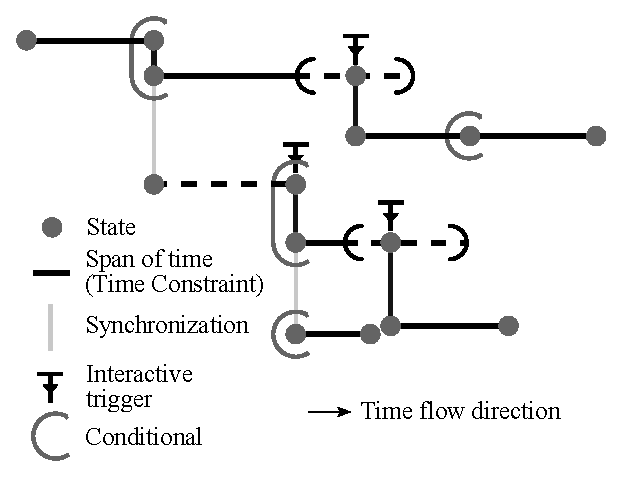
\includegraphics[width=0.45\textwidth]{figures/iscore-example.eps}
	\caption{Part of an i-score scenario, showcasing the temporal syntax used. 
		A full horizontal line means that the time must not be interrupted, 
		while a dashed horizontal line means that the time of this Constraint can be interrupted to proceed 
		to the following parts of the score according to an interactive event.}
	\label{fig.iscore-example}
\end{figure}

\subsection{Description LibAudioStream}
-> donner sémantique des flux.
-> players
-> donner example flux stream avec effet faust.
\section{Audio authoring in i-score}

\section{Presentation of the audio system}
In this section, we will explain the audio routing 
features offered by the software.

First, we introduce new audio streams that allow a LibAudioStream
expression to encapsulate the execution of a virtual audio player, 
in order to allow for hierarchy.

We make the choice to allow for hierarchy by mixing the played streams together.
This is done in accordance with the principle of least astonishment\cite{seebach2001cranky} for the composer : 
in most audio software, the notion of grouping implies that the grouped sounds will be mixed 
together and routed to a single audio bus.

Then, we present the concept of audio buses integrated to the LibAudioStream,
with two special Send and Return streams.

\subsection{Group audio stream}
In order to be able to apply hierarchical effects on the streams, 
we have to introduce a way to use hierarchy in the LibAudioStream.

Two elements are necessary : 
\begin{itemize}
	\item A particular audio player that will be able to sequence the starting and stopping 
	of interactive sounds.
	Such players already exist in the LibAudioStream but are tailored for direct output to
	the soundcard.
	\item A way to introduce the Renderer into the stream system, so that it 
	is able to be pulled like it would be by a real soundcard.
\end{itemize}

We introduce two matching objects in the LibAudioStream~: 
\begin{itemize}
	\item A Group player. This is a player whose processing function has to be called manually. 
	Timekeeping supposes that it will be pulled in accordance at the clock rate
	and samplerate of the soundcard.
	\item A Group audiostream. This particular audiostream, of infinite length, 
	allows to introduce a Group player in a series of chained streams.
	For instance~:~\\\lstinline[language=LISP]{(mix (fx playerA fxA) (fx playerB fxB))}
\end{itemize}

The execution time of the hierarchized objects will be relative to the start time of the Group audiostream.
The sound of the objects will be mixed together.

\subsection{Send and return audio streams}
In order to be able to create rich effect graphs, we introduce another couple of objects.

The Send audiostream by itself is a passthrough : it just pulls the stream it owns.
It posseses the same definition : same length, same number of channels\dots
The Return audiostream, constructed with a Send stream, will make a copy of the data in 
the send stream and allow it to be used by the processing chain it is part of.
This means that a sound source can be sent to sound effects in parallel, for instance.

The Return stream is infinite in length : to allow for long-lasting audio effects 
like reverb queues or delays, we suppose that we can pull the data from the Send stream at any point in time.
If a Return stream tries to fetch the data of a Send stream that has not started yet, or that has already finished, a buffer of silence is provided instead.

A byproduct of the imposed acyclicity of the graph, some level of parallel processing may be achieved, as long as causality is respected between nodes. 
For instance, if two Returns with each their own effect chain are connected to a Send, it is possible to compute these returns on different threads after the current buffer of the Send has been processed.

An important point is that the Send stream must itself be pulled regularly by being played as a sound, either directly or by a stream that would encapsulate it.

\begin{figure}
	\centering
	\includegraphics[width=0.45\textwidth]{figures/graph2.eps}
	\caption{Possible mixing with the Send and Return objects. An arrow from A to B means that B pulls the audio data from A.}
	\label{fig.mixsendreturn}
\end{figure}

\subsection{Audio processes}
We provide multiple audio processes in i-score, that map 
to lower-level audio streams.

\begin{itemize}
	\item Effect chain process : register multiple audio effects one after the other. 
	For instance~:~\\ \emph{ Equalizer $\,\to\,$ Distortion $\,\to\,$ Reverb}. ~\\
	Currently only Faust effects are supported.
	\item Generator process : a sound generator, like a synthesizer. 
	Currently only Faust instruments are supported.
	\item Sound file.
	\item Explicit send and return processes.
	\item Mixing process.
\end{itemize}

An important feature of audio workstations is the support for automation, that is, 
controlling the value of a parameter over time, generally with piecewise continuous functions.
In i-score automation is generally achieved by sending OSC messages to a remote software;
the OSC message tree is modeled as an object tree.
We introduce the loaded effect plug-in to this object tree, so that automations 
and mappings are able to control audio effects and audio routing parameters such as volume.

An example is given in fig.~\ref{fig.iscoreconstraint}.
\begin{figure}
	\centering
	\includegraphics[width=0.25\textwidth]{figures/iscore1.eps}
	\caption{An example of a Time Constraint loaded with audio processes in i-score. 
		Selecting a particular process shows a complete widget for editing the parameters.}
	\label{fig.iscoreconstraint}
\end{figure}
\subsection{Stream graph}
One problem caused by the presence of routing is that it is possible 
to create a data loop : if a Send is directly or indirectly fed its own data through a Return, 
the output would be garbage data : the Return would be asked to read 
the currently requested output from the Send which has not been written yet.

To prevent this, we create a graph where : 
\begin{itemize}
	\item Vertices are the sound generating elements : audio file reader, etc.
	\item Edges are the connections going from a send to a return.
\end{itemize} 

The graph, implemented with the Boost Graph Library~\cite{siek2001boost} can then be used to 
guarantee the acyclicity, and return an user error if that is not the case.

We provide here the algorithm to build the graph.

\todo{Disambiguate the user-created sends and the sends required for the model}
%\paragraph{Vertice creation}
Vertices are created recursively from the Time Constraints in i-score.
First, we iterate through all the processes of the given constraint.
If the process is hierarchical (Scenario, Loop), then we call the algorithm recursively on the process.
In the case of the Scenario, it means that we call recursively on all its Constraints; in the case of the Loop, we call recursively on its loop pattern Constraint.
In both case, we create a Group vertice to model the process.
Then, we create inner Sends for all the streams and a vertice for the Constraint itself.

\begin{figure}
	\centering
	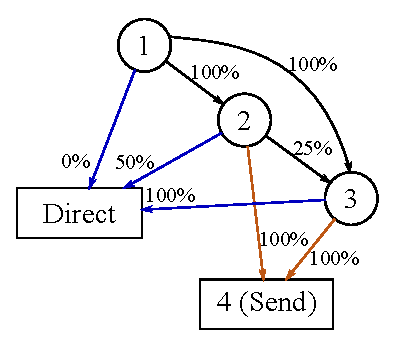
\includegraphics[width=0.35\textwidth]{figures/graph1.eps}
	\caption{Translation of the Time Constraint of fig.~\ref{fig.iscoreconstraint} in a dependency graph.
		The edges in black represent the intra-Constraint connections. 
		The edges in blue (resp. orange) represent a connection to a visible output of 
		the Constraint. The percentages represent the level of mixing of the stream.
		\textit{Direct} corresponds to the signal that will be sent at the upper level of hierarchy.}
	\label{fig.graph}
\end{figure}

As can be seen, there can be an ordering between nodes of the graph : the parentmost vertice
has to be pulled before the others to reflect the causality.
\todo{Comparer à Ableton ou il est possible pour chaque piste de choisir son entrée et sa sortie.}

Inside a Time Constraint, causality also has to be enforced. 
Since a mixing bus is provided, we have to ensure that an effect bus cannot be routed in 
itself in a loop. 
To prevent this at the user interface level, the vertical order of effect chains is used : 
if Effect Chain 1 comes before Effect Chain 2, then Effect Chain 1 can be routed into Effect Chain 2, but not the contrary.

\todo{placement de la chaine de gain, time stretch, etc.}
\subsection{Stream creation}
\subsubsection{Scenario}
An i-score scenario is an arrangement of temporal structures, as shown in fig.~\ref{fig.iscore-example}.
Since the duration of these structures can change at run-time, it is not meaningful to use the tools provided by the LibAudioStream : sequence stream, parallel stream, mix stream.

\begin{enumerate}
	\item A Group player is created.
	\item For each Time Node in the scenario, a symbolic date is generated.
	\item For each Time Constraint in the scenario, a stream is built; it is started and stopped at the symbolic date matching its start and end Time Nodes in the group player.
\end{enumerate}

The Audio stream of this process is the group player.

\subsubsection{Loop}
Due to their interactive nature, loops in i-score can be entirely different from 
one iteration to another; they are more similar to traditional programming language \texttt{do-while} constructs, than audio sequencer loops.

- problème des boucles dans i-score : chaque itération peut être différente.
\subsubsection{Time Constraint}
\todo{audio-graphe pour contrainte avec duplication des effets}

-> donner sémantique de flux des Stream Group, Send, Return.

- Comme la durée de chaque contrainte peut varier avec le ralentissement, on utilise principalement 
des dates symboliques

Faire graphe pour une Time Constraint et donner un exemple avec effets appliqués sur scénario.
Expliquer graphe hiérarchique de dépendances : penser au cas ou un a un return dans une hiérarchie puis un send à un niveau supérieur; il faut faire le grpahe de A à Z et s'assurer qu'il ne soit pas cyclique

1er cas : 
Un son avec une piste d'effets.

2eme cas : scénario hiérarchique, boucle

Cas de la boucle avec un coup A, un coup B selon la condition ? 
-> exécution d'un timenode doit reset le flux.

Piste send / return : permet de maintenir les queues de reverb.


\subsection{Routing, multi-channels, etc.}
-> mettre maquettes track mix

\section{Example}
\subsection{UI}
-> capture d'écran
Faire vue scénario et sa traduction en graphe de routage 

\subsection{Temporal effect graphs}
\section{Conclusion}
-> lackluster areas : 
- MIDI support (but OSC)
- no musical time information : first aimed for artists, 
but improvements could be the waiting of triggering on some measure of time.
- "play from anywhere"
- audio input ?
- correction de latence ?
- pour l'instant pas d'optimisations dans des cas simples (e.g. pas besoin de mixage)
\begin{acknowledgments}
    ANRT, Blue Yeti, Magali
\end{acknowledgments} 

%%%%%%%%%%%%%%%%%%%%%%%%%%%%%%%%%%%%%%%%%%%%%%%%%%%%%%%%%%%%%%%%%%%%%%%%%%%%%
%bibliography here
\bibliography{smc2016template}

\end{document}
